\documentclass[xcolor=dvipsnames]{beamer}
\usepackage[utf8]{inputenc} 

\definecolor{LightGray}{gray}{0.75}

\usepackage{textcomp}

\usepackage{caption}
\usepackage{listings}
\makeatletter
\lstdefinestyle{smallstyle}{
  basicstyle=%
    \ttfamily
    \color{blue}%
    \scriptsize
}
\makeatother

\usepackage{caption}
\usepackage{listings}
\makeatletter
\lstdefinestyle{normalstyle}{
  basicstyle=%
    \ttfamily
    \color{blue}%
}
\makeatother

\lstset{style=smallstyle}

\usepackage{anyfontsize}

\usepackage[font=itshape]{quoting}
\quotingsetup{vskip=4pt} % vertical spacing of quotes


\usecolortheme{seahorse} %colour theme, cf https://www.hartwork.org/beamer-theme-matrix/

\title[] {Group 1.2 - Position Prediction}
\date{} % no date

% empty to have to numbering of split-up frames from allowframebreaks
% cf http://tex.stackexchange.com/questions/193308/how-can-we-change-allowframebreaks-numbering-in-the-title#212292
\setbeamertemplate{frametitle continuation}{}


\begin{document}

\begin{frame}
	\frametitle{\textbf{Position Prediction}~~--~~Group 1.2}
	\centering
	\includegraphics[width=0.6\textwidth]{stork.png}
\end{frame}

\begin{frame}
	\frametitle{\textbf{Workflow}~~(so far)}
	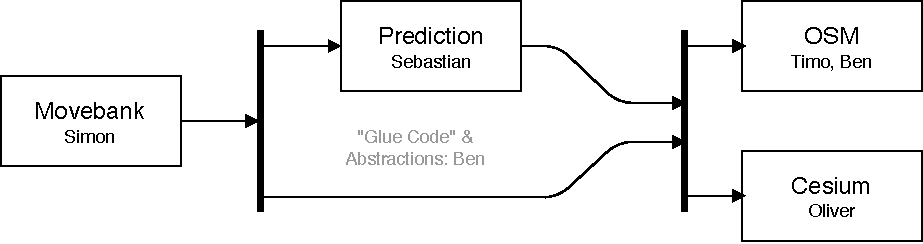
\includegraphics[width=\textwidth]{diagrams/Tasks.pdf}
\end{frame}

\begin{frame}
	\frametitle{\textbf{Software Design}~~--~~achieved so far}
	%
	\large{Milestone 1 (15.5.)}
	\normalsize
	\begin{itemize} 
		\item \color{Green}Grundliegende Software-Architektur festgelegt
		\item \color{Green}Grundliegendes Software-Design festgelegt
		\item \color{Green}Ein Grundgerüst der Applikation ist fertiggestellt: Es sind folgende Ansichten funktional umgesetzt:
		\begin{itemize} 
			\item \color{Green}Offline-Karten (eine Kartenumgebung wird angezeigt, Navigation möglich)
			\item \color{Green}Diverse UI-Elemente (mindestens Eingabefeld, Button)
		\end{itemize} 
		\item \color{LightGray}Die Positionsdaten für die Vorhersage werden von der \textit{Movebank}-API bezogen.
	\end{itemize}     
	%
	\large{Milestone 2 (5.6.)}
	\normalsize
	\begin{itemize} 
		\item \color{LightGray}Es wird eine Vorhersage mittels eines einfachen Vorhersagemodells berechnet.
		\item \color{LightGray}Es existiert eine funktionale Visualisierung des Vorhersage-Ergebnisses.
		\item \color{LightGray}Es existiert eine Möglichkeit, eine Cesium Ansicht von der Applikation aus aufzurufen.
		\item \color{Green}Der Aufbau des User-Interfaces ist festgelegt (nicht-funktionale Mockups).
	\end{itemize}
\end{frame}


\begin{frame}
	\frametitle{\textbf{Software Architecture I}~~--~~achieved so far}
	\begin{columns}
	\begin{column}{0.5\textwidth}
		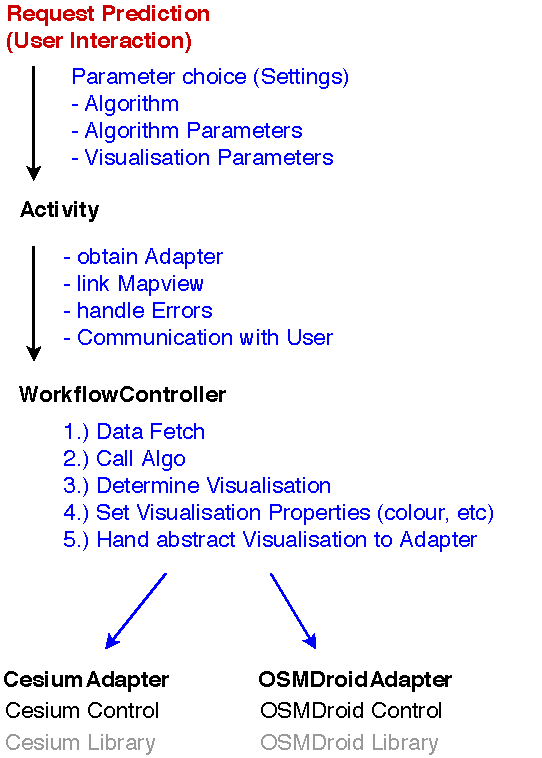
\includegraphics[width=\textwidth]{diagrams/controller-flow.pdf}
	\end{column}
	\begin{column}{0.5\textwidth}
		\fontsize{9pt}{9}\selectfont
		Benefits:
		\begin{itemize}
		 	 \item Easier to write: Controller doesn't care about Algo or Map implementation
		 	 \item Easier to integrate (call from anywhere)
		 	 \item Highly extensible (could subclass controllers?)
		 	 \item Same code for visualisation of past and predicted locations {\tiny(assumption: never want to see data without a prediction $\rightarrow$ AnimalTracker)}
		\end{itemize}
 	\end{column}
	\end{columns}
\end{frame}

\begin{frame}
	\frametitle{\textbf{Software Architecture II}~~--~~achieved so far}
	\begin{columns}
	\begin{column}{0.5\textwidth}
		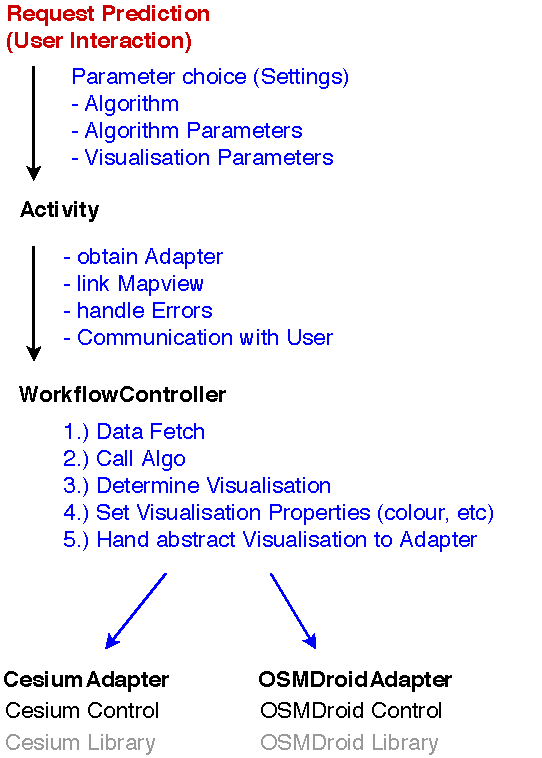
\includegraphics[width=\textwidth]{diagrams/controller-flow.pdf}
	\end{column}
	\begin{column}{0.5\textwidth}
		\fontsize{9pt}{7.2}\selectfont
		Challenges:
		\begin{itemize}
			\item Separation of Concerns, D.R.Y.
		 	 \item How to model data in a general but still meaningful, usable, maintainable way?
		 	 \begin{itemize}
		 	 	\item e.g. Types \lstinline$Locations > SingleTrajectory$, \lstinline$SingleTrajectoryVis$, \lstinline$AlgParams$
		 	 \end{itemize}
		\end{itemize}
 	\end{column}
	\end{columns}
\end{frame}


\begin{frame}
	\frametitle{\textbf{Software Architecture III}~~--~~achieved so far}
	\begin{columns}
	\begin{column}{0.5\textwidth}
		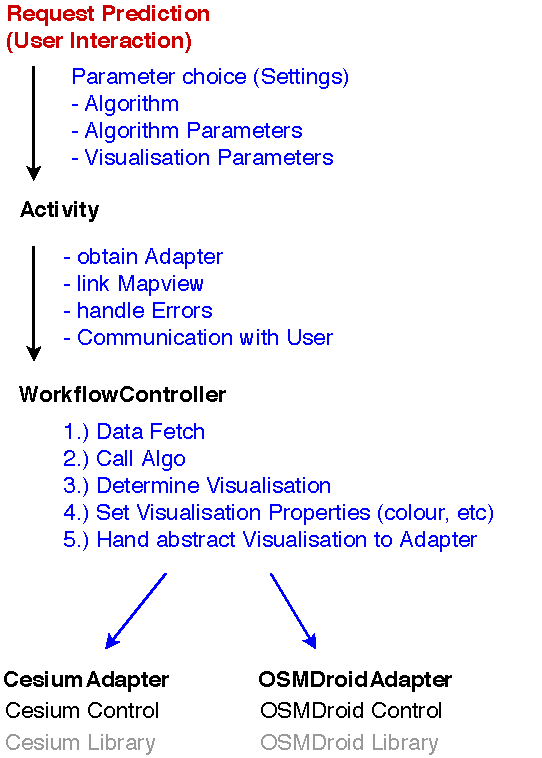
\includegraphics[width=\textwidth]{diagrams/controller-flow.pdf}
	\end{column}
	\begin{column}{0.5\textwidth}
		\fontsize{9pt}{7.2}\selectfont
		\begin{itemize}
		 	 \item \lstinline$OSMDroidAdapter$: Convert data to OSM-specific Types and call the right drawing methods.
		 	 \item \lstinline$OSMDroidMap$: Library specific code %
		 	 \begin{itemize}
		 	  	 \item enable features
		 	  	 \item draw stuff
		 	  	 \item handle events
		 	  	 \item make undocumented library functions usable
		 	 \end{itemize}
		\end{itemize}
 	\end{column}
	\end{columns}
\end{frame}


\begin{frame}
	\frametitle{\textbf{Software Architecture IV}~~--~~next steps}
	How to integrate...
	\begin{itemize}
		\item ... error handling? (throw where, catch where?)
		\item ... user communication? (error messages, progress bars...)
	\end{itemize}
	\lstset{style=normalstyle}
	\begin{itemize}
		\item Achieve higher generality in \lstinline$WorkflowController$
	\end{itemize}
	\begin{itemize}
	 	 \item ... see project timeline.
	\end{itemize}
\end{frame}




\begin{frame}
	\frametitle{\textbf{Movebank}~~--~~achieved so far}
	\Large{Milestone 1 (15.5.)}
	\normalsize
	\begin{itemize} 
		\item \color{LightGray}Grundliegende Software-Architektur festgelegt
		\item \color{LightGray}Grundliegendes Software-Design festgelegt
		\item \color{LightGray}Ein Grundgerüst der Applikation ist fertiggestellt: Es sind folgende Ansichten funktional umgesetzt:
		\begin{itemize} 
			\item \color{LightGray}Offline-Karten (eine Kartenumgebung wird angezeigt, Navigation möglich)
			\item \color{LightGray}Diverse UI-Elemente (mindestens Eingabefeld, Button)
		\end{itemize} 
		\item \color{Green}Die Positionsdaten für die Vorhersage werden von der \textit{Movebank}-API bezogen.
	\end{itemize}     
\end{frame}




\begin{frame}
	\frametitle{\textbf{Internal Database}~~--~~achieved so far}
    
	\begin{itemize}
		\item CSV-Files from the Movebank are parsed and the data is put into the Database.
		\item Data can be accessed using SQL queries
	\end{itemize}
    
\end{frame}



\begin{frame}
	\frametitle{\textbf{Prediction I}~~--~~achieved so far}
	%
	\large{Milestone 2 (5.6.)}
	\normalsize
	\begin{itemize} 
		\item \color{Green}Es wird eine Vorhersage mittels eines einfachen Vorhersagemodells berechnet.
		\item \color{LightGray}Es existiert eine funktionale Visualisierung des Vorhersage-Ergebnisses.
		\item \color{LightGray}Es existiert eine Möglichkeit, eine Cesium Ansicht von der Applikation aus aufzurufen.
		\item \color{LightGray}Der Aufbau des User-Interfaces ist festgelegt (nicht-funktionale Mockups).
	\end{itemize}
\end{frame}

\begin{frame}
	\frametitle{\textbf{Prediction II}~~--~~achieved so far}
	\Large{AlgorithmExtrapolationExtended}
	\normalsize{}
			\begin{itemize}
				\item[(+)] Good if the variance of the angles is not too big
				\item[(+)] Later datapoints are weighted more
				\item[(+)] Fast
				\item[(+)] Easy to understand
				\item[] 
				\item[( - )] Not very accurate
				\item[( - )] Early data gets ignored

			\end{itemize}
\end{frame}

\begin{frame}
	\frametitle{\textbf{Prediction III}~~--~~achieved so far}
	\Large{AlgorithmSimilarTrajectory}
	\normalsize{}
			\begin{itemize}
				\item[(+)] Good if the measuring frequency is high
				\item[(+)] Earlier datapoints are important for the result
				\item[(+)] Multiple trajectories can be found
				\item[(+)] Easy to understand
				\item[] 
				\item[( - )] Frequency is not always high $\Rightarrow$ Wrong result
				\item[( - )] Higher complexity than the other algorithm
				\item[( - )] (Currently) only works with the same time span between datapoints
			\end{itemize}
\end{frame}



\begin{frame}
	\frametitle{\textbf{Visualization (OSM) I}~~--~~achieved so far}
	%
	\large{Milestone 2 (5.6.)}
	\normalsize
	\begin{itemize} 
		\item \color{LightGray}Es wird eine Vorhersage mittels eines einfachen Vorhersagemodells berechnet.
		\item \color{Green}Es existiert eine funktionale Visualisierung des Vorhersage-Ergebnisses.
		\item \color{LightGray}Es existiert eine Möglichkeit, eine Cesium Ansicht von der Applikation aus aufzurufen.
		\item \color{LightGray}Der Aufbau des User-Interfaces ist festgelegt (nicht-funktionale Mockups).
	\end{itemize}
\end{frame}



\begin{frame}
	\frametitle{\textbf{Visualization (OSM) II}~~--~~mock-ups}
	\begin{columns}
	\begin{column}{0.5\textwidth}
		Geometric primitives\\
		(points, lines, polygons)
		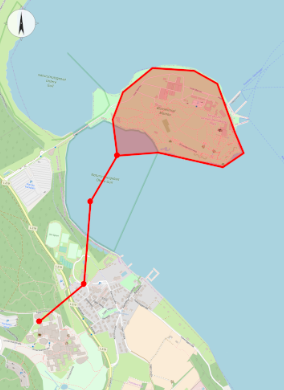
\includegraphics[width=\textwidth]{screenshots/vis-functional-1.png}
	\end{column}
	\begin{column}{0.56\textwidth}
		Real data
		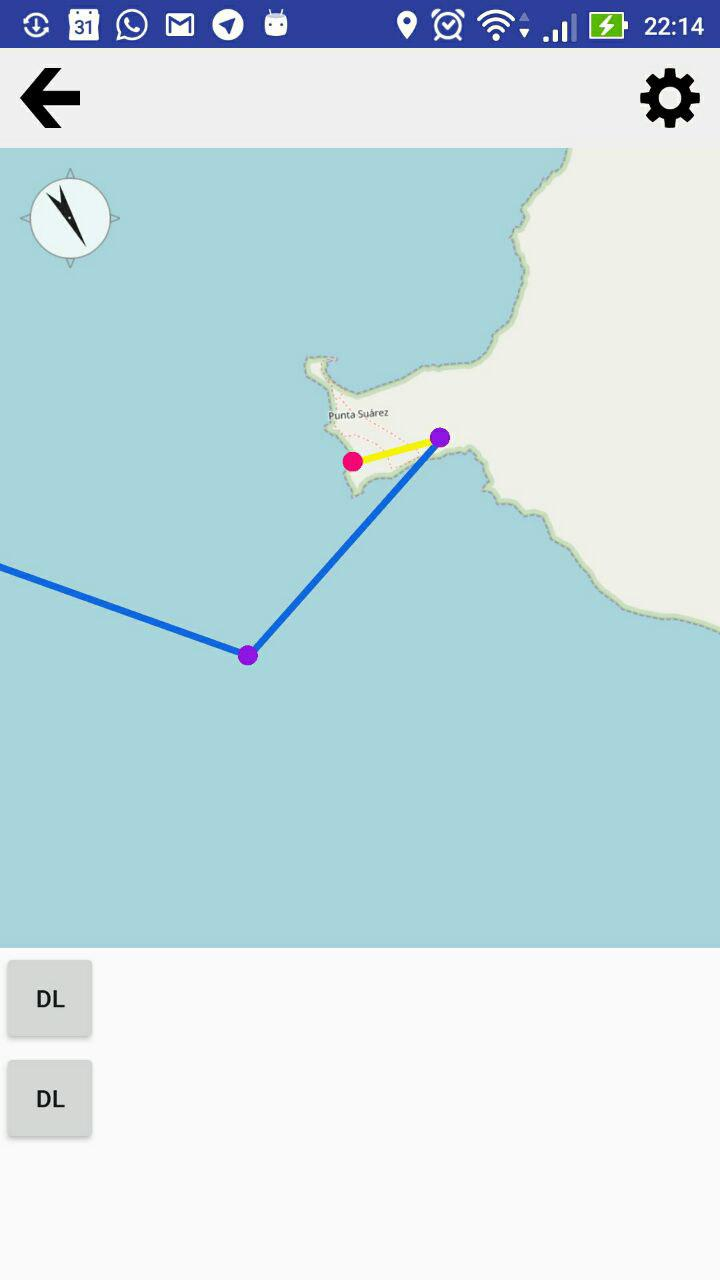
\includegraphics[width=\textwidth]{screenshots/vis-functional-2.jpg}
	\end{column}
	\end{columns}
\end{frame}


\begin{frame}
	\frametitle{\textbf{Visualization (OSM) III}~~--~~implementation}
		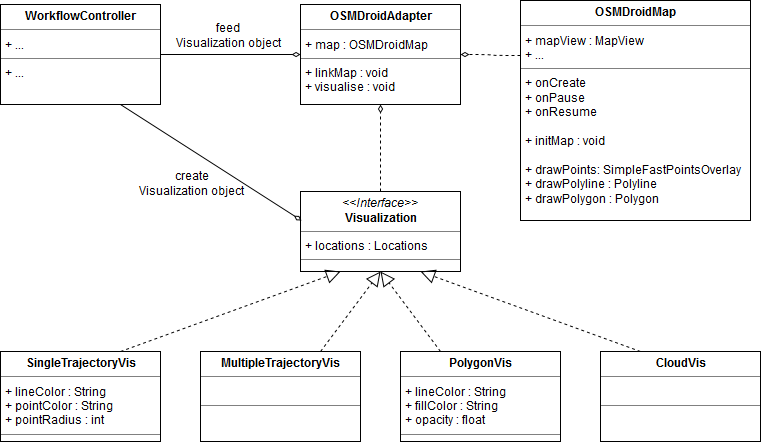
\includegraphics[width=\textwidth]{diagrams/ClassDiagram_OSM.png}
\end{frame}



\begin{frame}
	\frametitle{\textbf{Visualization (OSM) IV}~~--~~next steps}
	%
	\begin{itemize} 
		\item Design suitable visualizations for different types of\\ prediction output (trajectories, clouds, ...)
		\item Speed improvements
		\item Alternative map tile sources
		\item Improve visualisation readability
		\begin{itemize}
			\item On low zoom levels: cluster points without losing information \textit{(cf Example)}
			\item (Idea) Visualise time (e.g. map to point opacity)
			\item (Idea) Visualise speed (e.g. map to line segment colour)
			\item ...
		\end{itemize}		
	\end{itemize} 
\end{frame}

\begin{frame}
	\frametitle{\textbf{Visualization (OSM) V}~~--~~next steps: readibility}
	Low zoom levels leave out information:
	\begin{columns}
	\begin{column}{0.5\textwidth}
		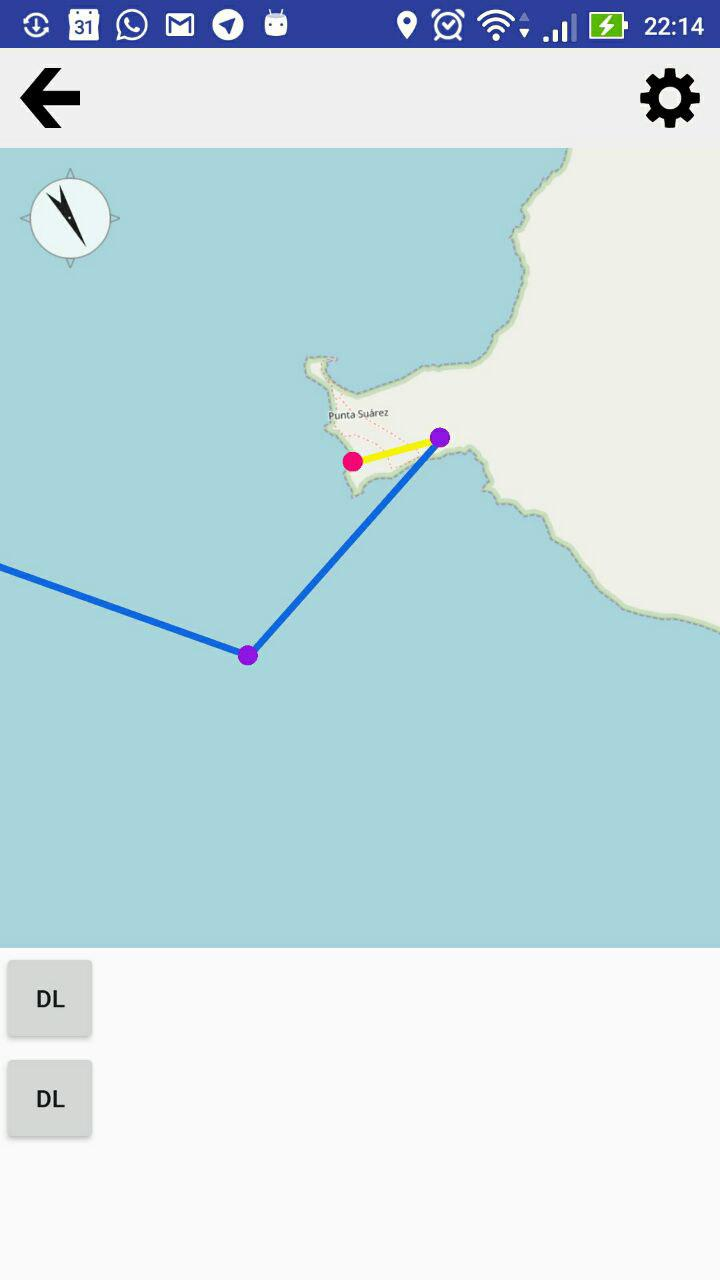
\includegraphics[width=1\textwidth]{screenshots/vis-functional-2.jpg}
	\end{column}
	\begin{column}{0.5\textwidth}
		\begin{center}
		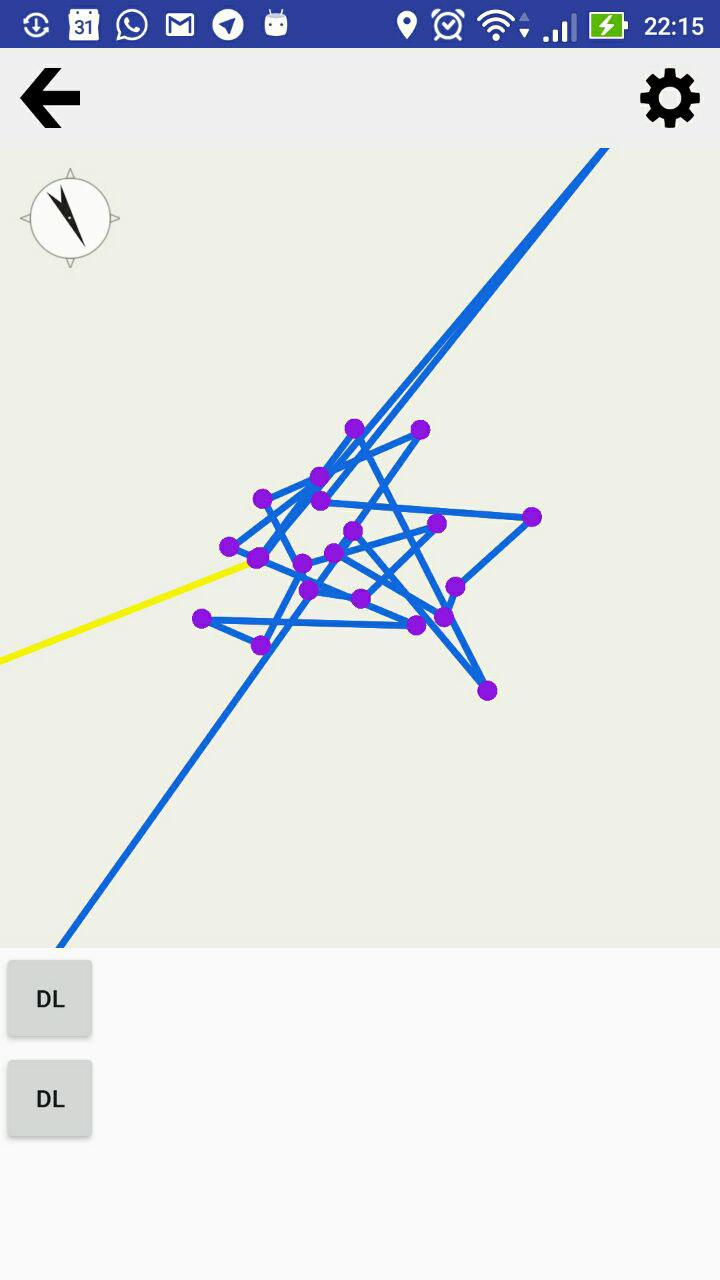
\includegraphics[width=1\textwidth]{screenshots/vis-readability-2.jpg}
		\end{center}
	\end{column}
	\end{columns}
\end{frame}


\begin{frame}
	\frametitle{\textbf{Visualization (Cesium) I}~~--~~achieved so far}
	%
	\large{Milestone 2 (5.6.)}
	\normalsize
	\begin{itemize} 
		\item \color{LightGray}Es wird eine Vorhersage mittels eines einfachen Vorhersagemodells berechnet.
		\item \color{LightGray}Es existiert eine funktionale Visualisierung des Vorhersage-Ergebnisses.
		\item \color{Green}Es existiert eine Möglichkeit, eine Cesium Ansicht von der Applikation aus aufzurufen.
		\item \color{LightGray}Der Aufbau des User-Interfaces ist festgelegt (nicht-funktionale Mockups).
	\end{itemize} 
\end{frame}

\begin{frame}
	\frametitle{\textbf{Visualization (Cesium) II}~~--~~achieved so far}
	\begin{columns}
	\begin{column}{0.5\textwidth}
		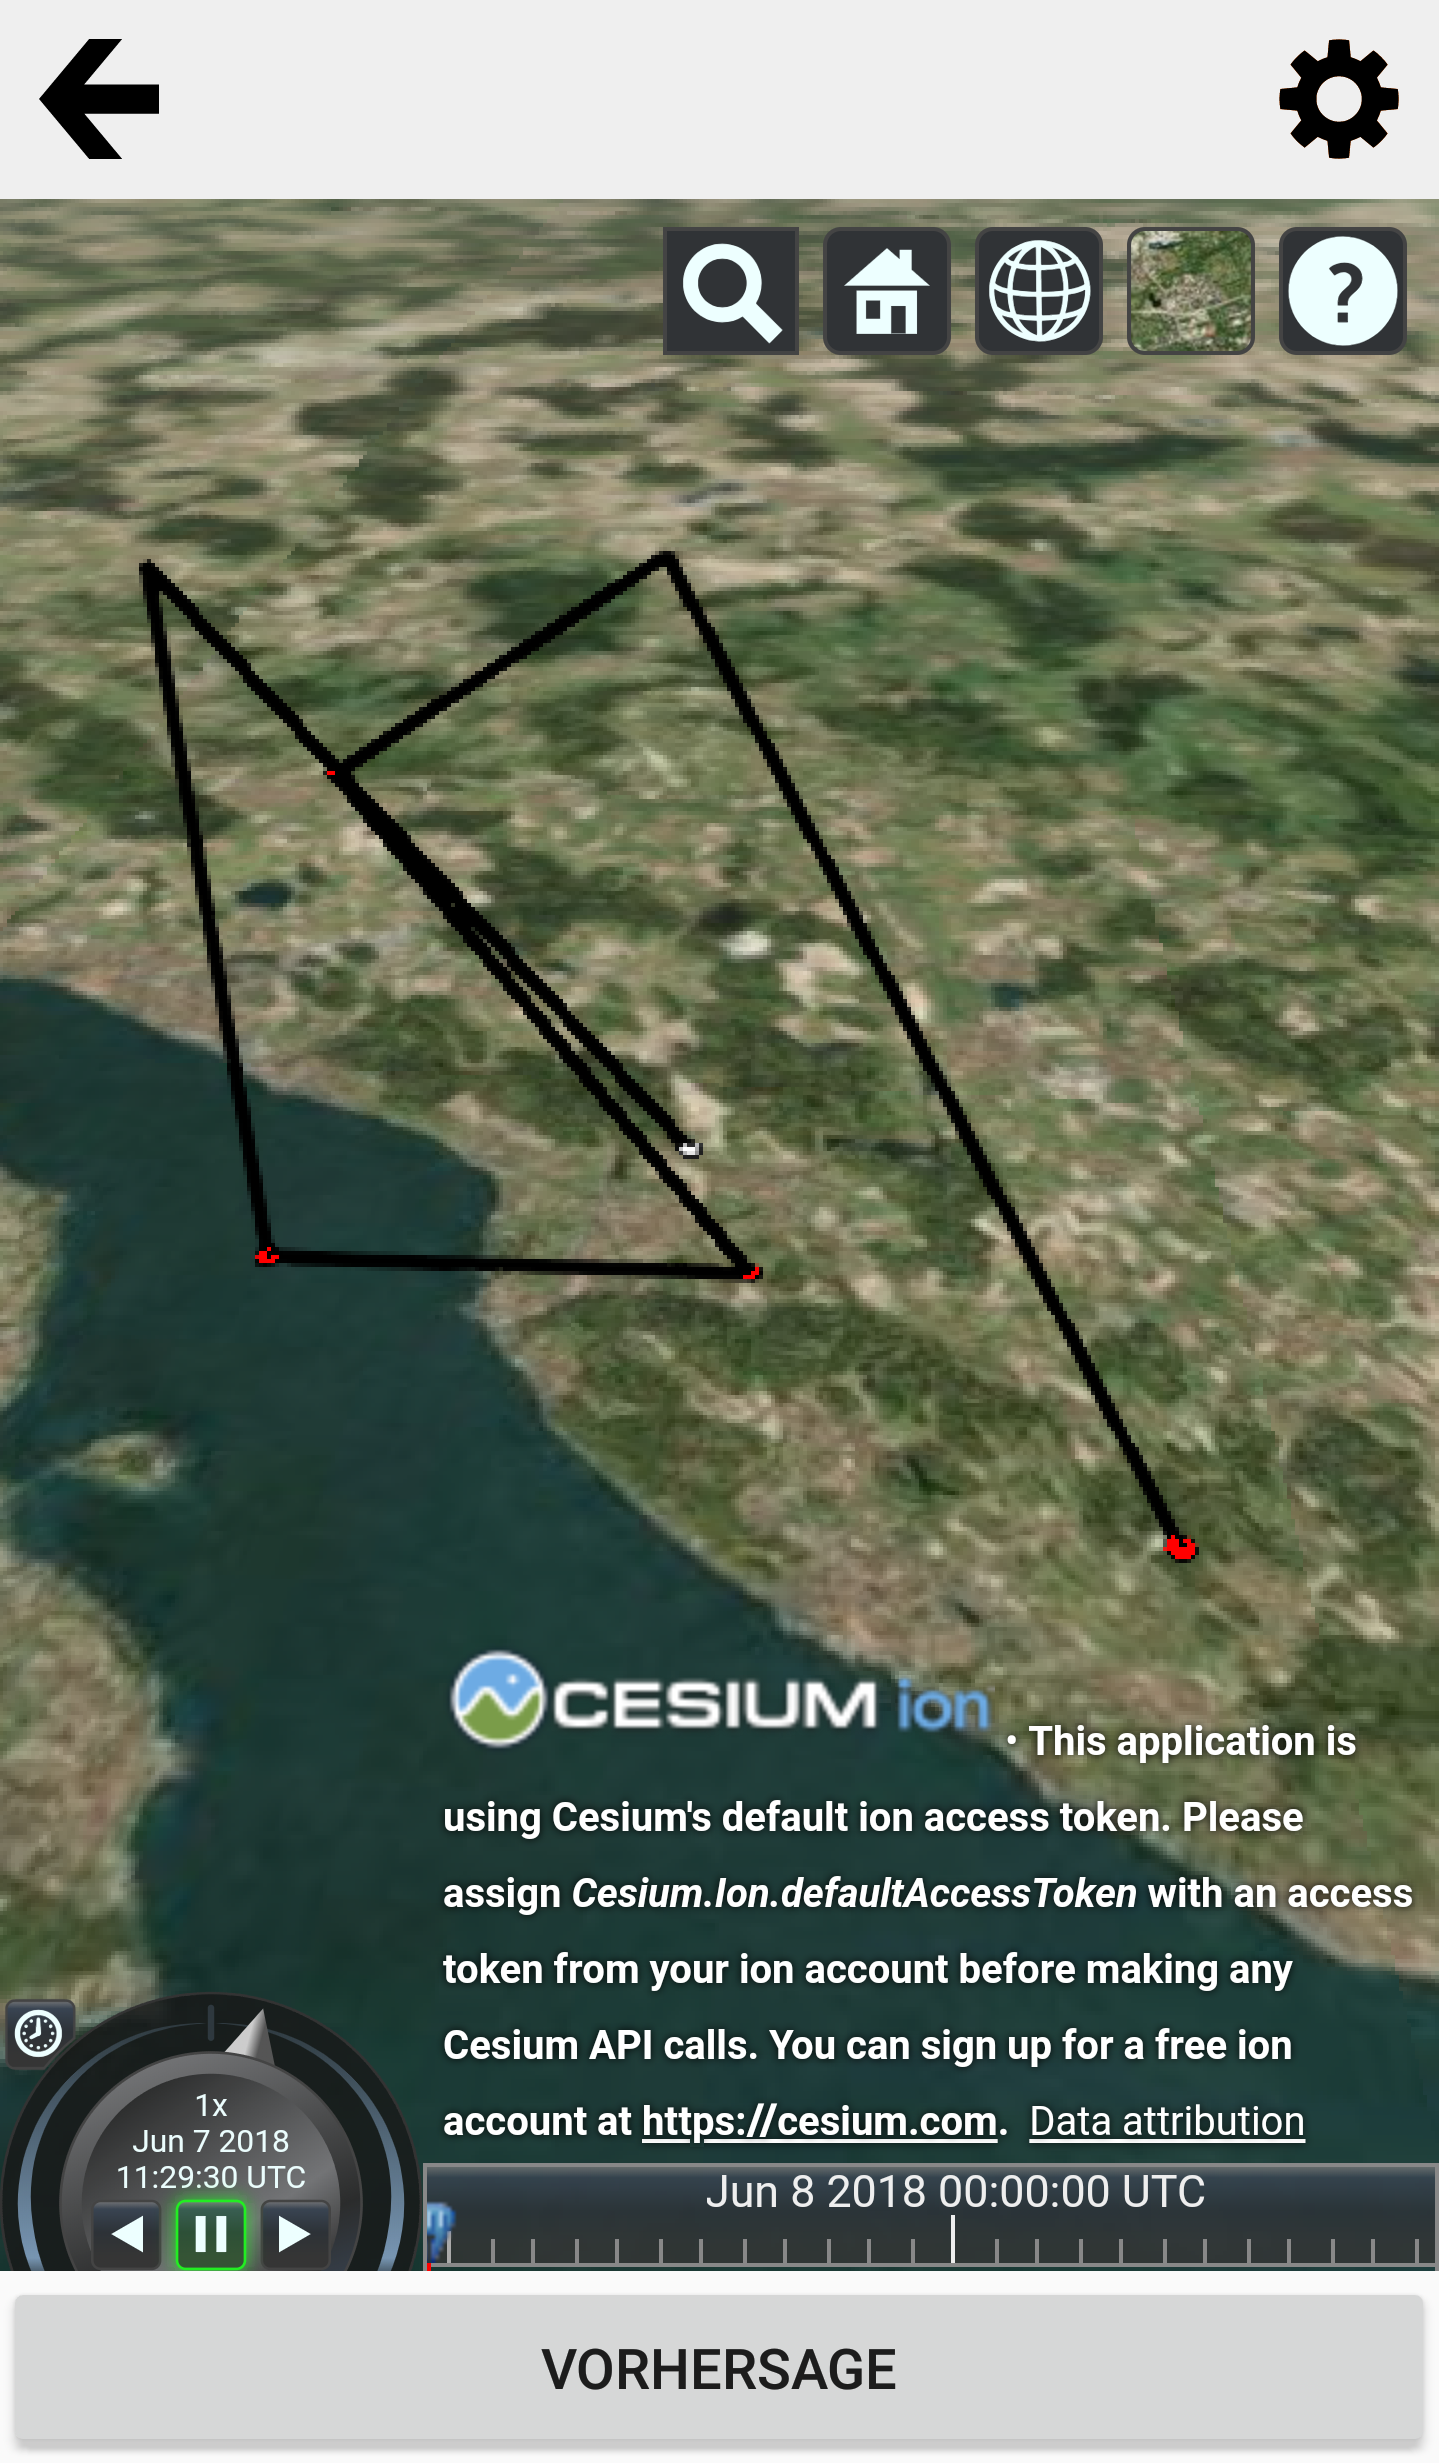
\includegraphics[width=0.8\textwidth]{screenshots/cesium-prediction1.png}
	\end{column}
	\begin{column}{0.5\textwidth}
		\begin{center}
		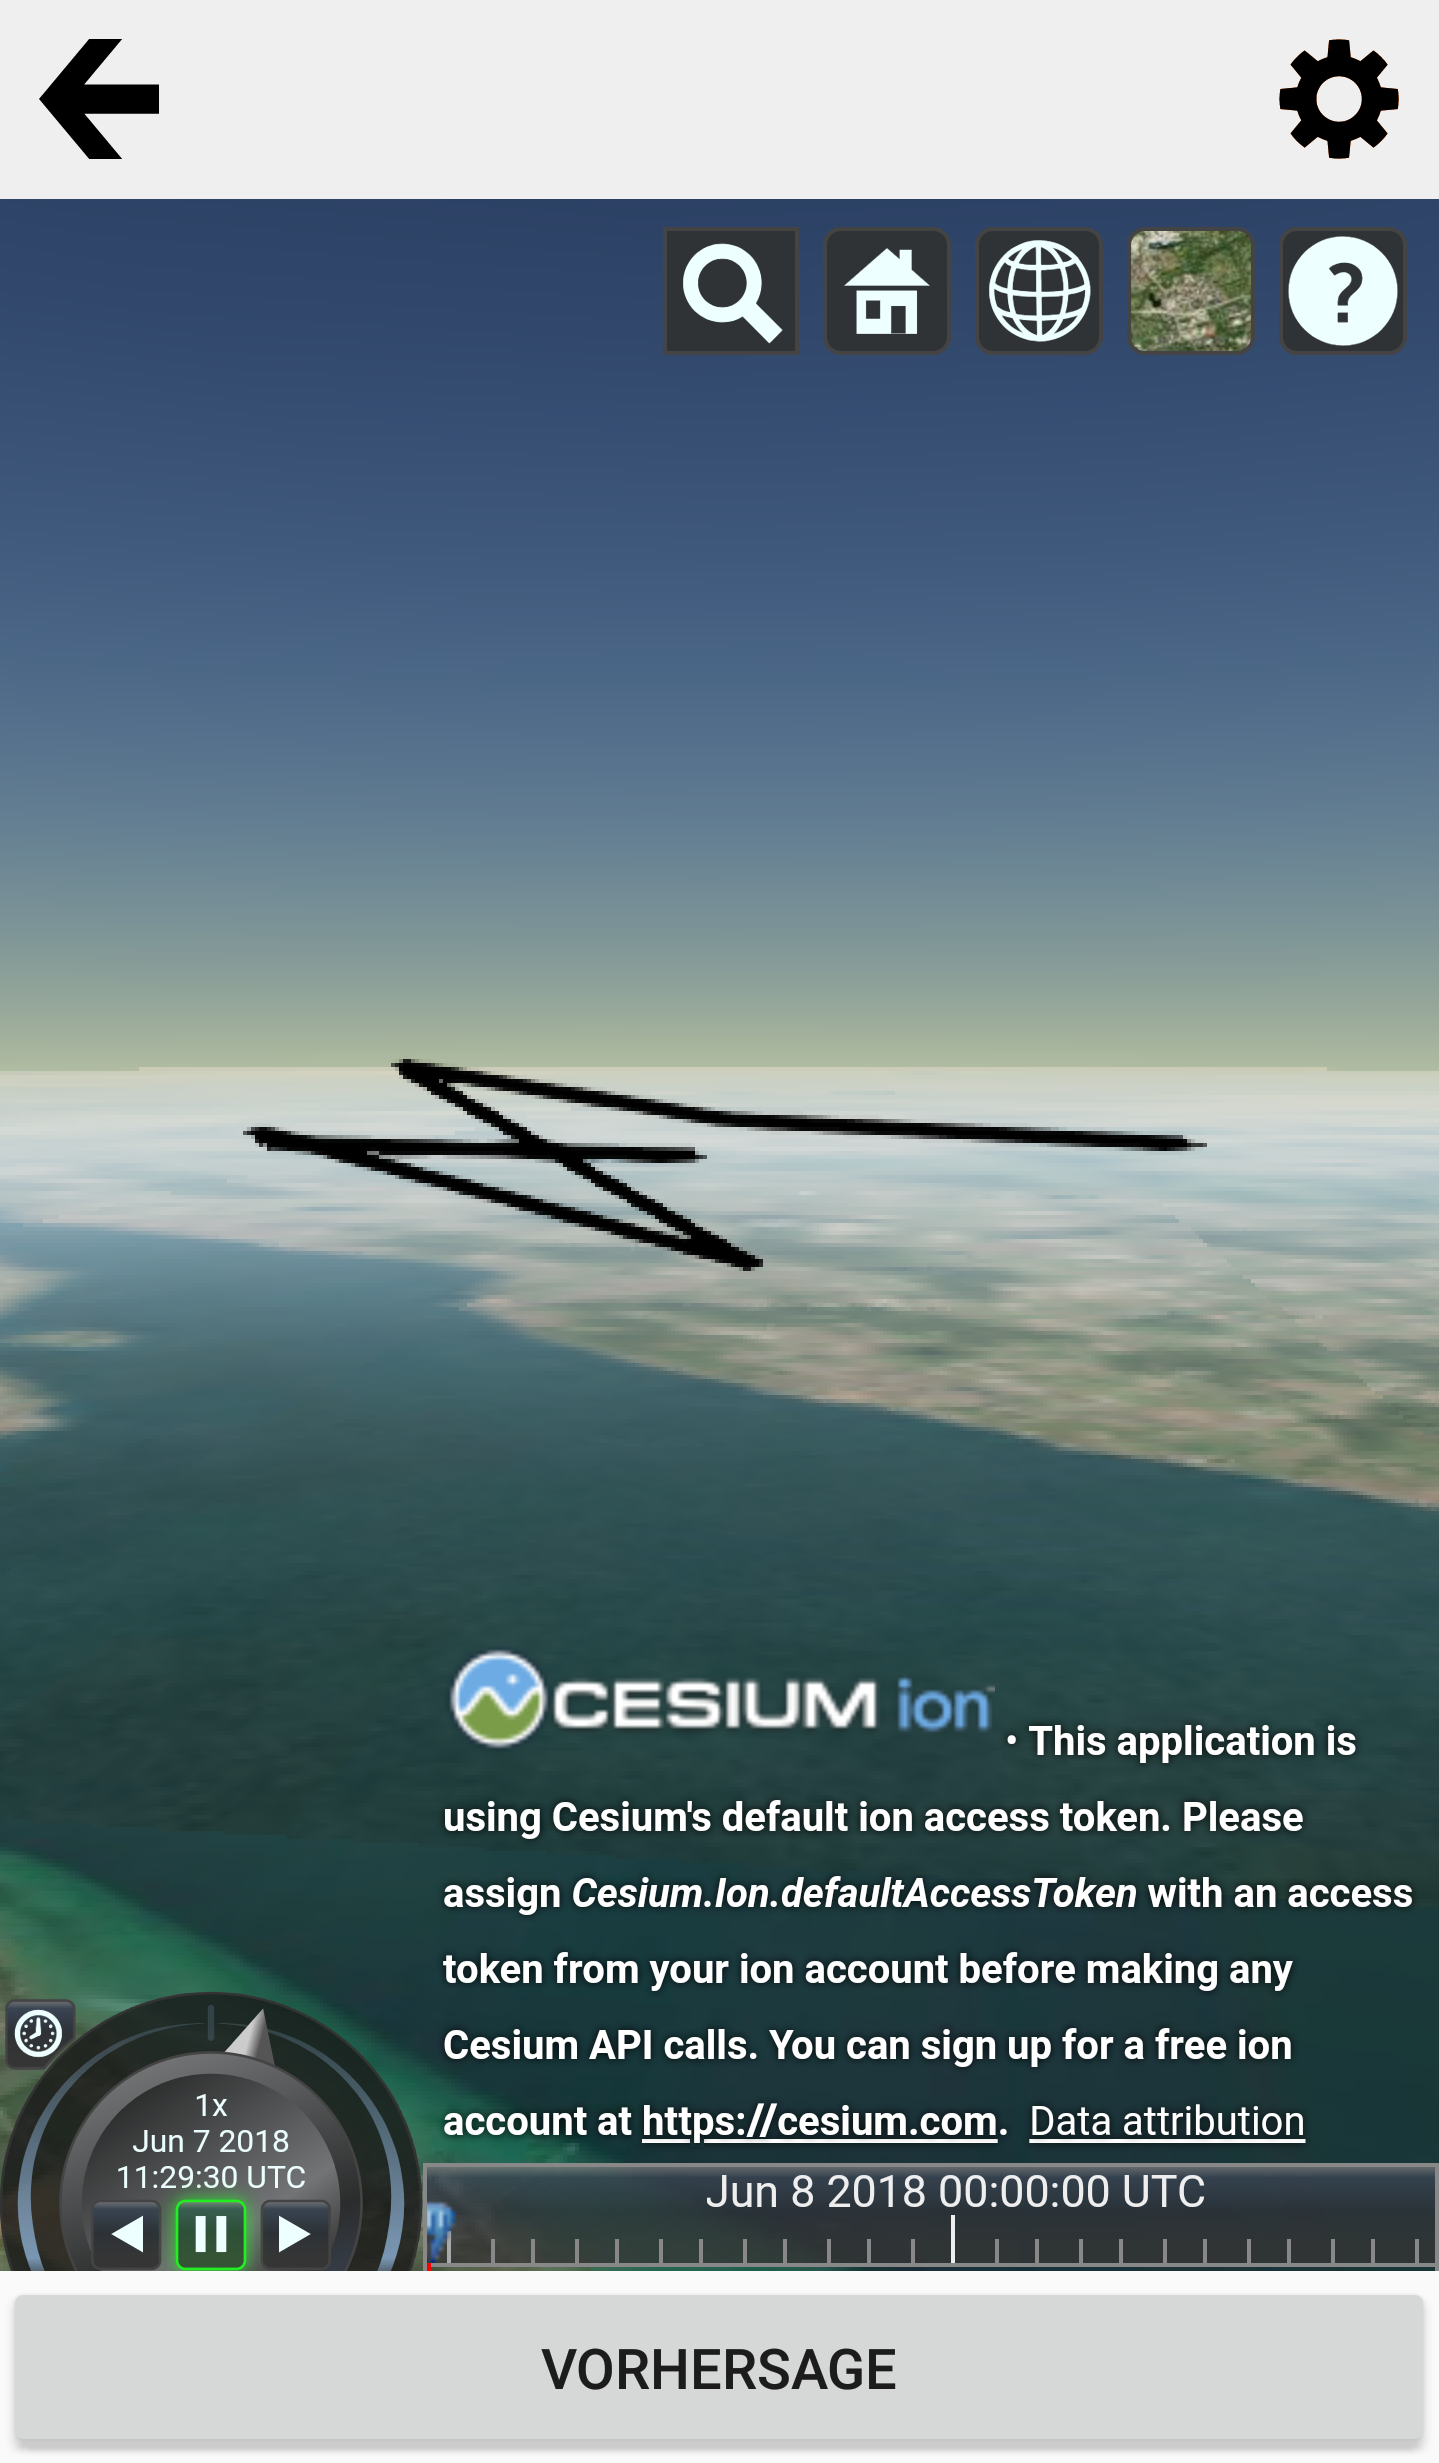
\includegraphics[width=0.8\textwidth]{screenshots/cesium-prediction2.png}
		\end{center}
	\end{column}
	\end{columns}
\end{frame}


\begin{frame}
	\frametitle{\textbf{Project timeline I}}
	%
	\Large{Woche 1 (07.-15.05.)}
	\normalsize
	~\\
	\begin{itemize}
		\item \color{Green} Grundgerüst der Applikation
		\item \color{Green} Daten von der \textit{Movebank}-API abfragen
		\item \color{Green} \textit{Software Design Document} verfassen
		\item \color{Green} \textbf{Milestone 1} erreicht
	\end{itemize}
	~\\
	\Large{Woche 2 (15.-22.05.)}
	\normalsize		
	~\\
	\begin{itemize}
		\item \color{Green} Daten verarbeiten (Movebank, Robustheit berücksichtigen) 
		\item \color{Green} Darstellung einer 2D-Karte \\
		\item \color{Green} Vorhersagemethode und -Interface implementieren
	\end{itemize}
	~\\		
	%
	\Large{Woche 3 (22.-29.05.)}
	\normalsize
	~\\
	\begin{itemize}
		\item \color{Green} Dummy-Visualisierung auf 2D-Karte \\
		\item \color{Green} Ergebnis der Vorhersage wird visualisiert. \\
		\item \color{Green} Visualisierung von Daten aus der Vergangenheit
	\end{itemize}	
\end{frame}

\begin{frame}
	\frametitle{\textbf{Project timeline II}}
	%
	\Large{Woche 4 (29.05.-05.06.)}
	\normalsize		
	~\\
	\begin{itemize}
		\item \color{Green} Cesium-Integration
		\item \color{Green} Speicherung von Kartendaten
		\item \color{Green} Datenvis. in Cesium
		\item \color{Green} \textbf{Milestone 2} erreicht
	\end{itemize}			
	~\\
	%
	\Large{Woche 5 (05.-12.06.)}
	\normalsize		
	~\\
	\begin{itemize}
		\item \color{Green} Suche nach Vogel
		\item \color{Green} Akt. Position auf Karte
		\item \color{Red} Speicherung von Mb-Nutzerdaten
	\end{itemize}		
	~\\
	%
	\Large{Woche 6 (12.-19.06.)}
	\normalsize		
	~\\
	\begin{itemize}
		\item \color{Red} Modi 
		\item \color{Red} Auswahl des Vorhersagezeitraums
		\item \color{Red} Auswahl von Daten für die Vorhersage
	\end{itemize}		
\end{frame}


\end{document}
